\chapter{Présentation et premiers programmes}

\section{Présentation pour la journée du patrimoine de l'IRISA}

\par
Olivier m'a proposé de réaliser \textbf{un diaporama} pour le stand de l'équipe Percept lors de la journée du patrimoine à l'IRISA programmé le 24 Mars 2020 à l'origine mais qui a été reportée à cause du contexte actuel de crise sanitaire. J'ai tout de même réalisé la présentation et devrait être diffusée à la prochaine journée du patrimoine. Olivier m'a conseillé de réaliser le diaporama en \LaTeX{} qui est un langage de programmation qui permet de réaliser des documents équivalents à ceux édités sous Word ou Open Office. L'avantage de ce langage est qu'il permet d'automatiser beaucoup d'élément, notamment la mise en page. Dans ma présentation je devais mettre une dizaine d'\oe{}uvres avec pour chacune d'elle une bonne quantité d'information (description, carte de saillance...). \LaTeX{} m'a permis d'automatiser la mise en diapositive des peintures pour un rendu de qualité.

\begin{figure}[!ht]
    \centering
    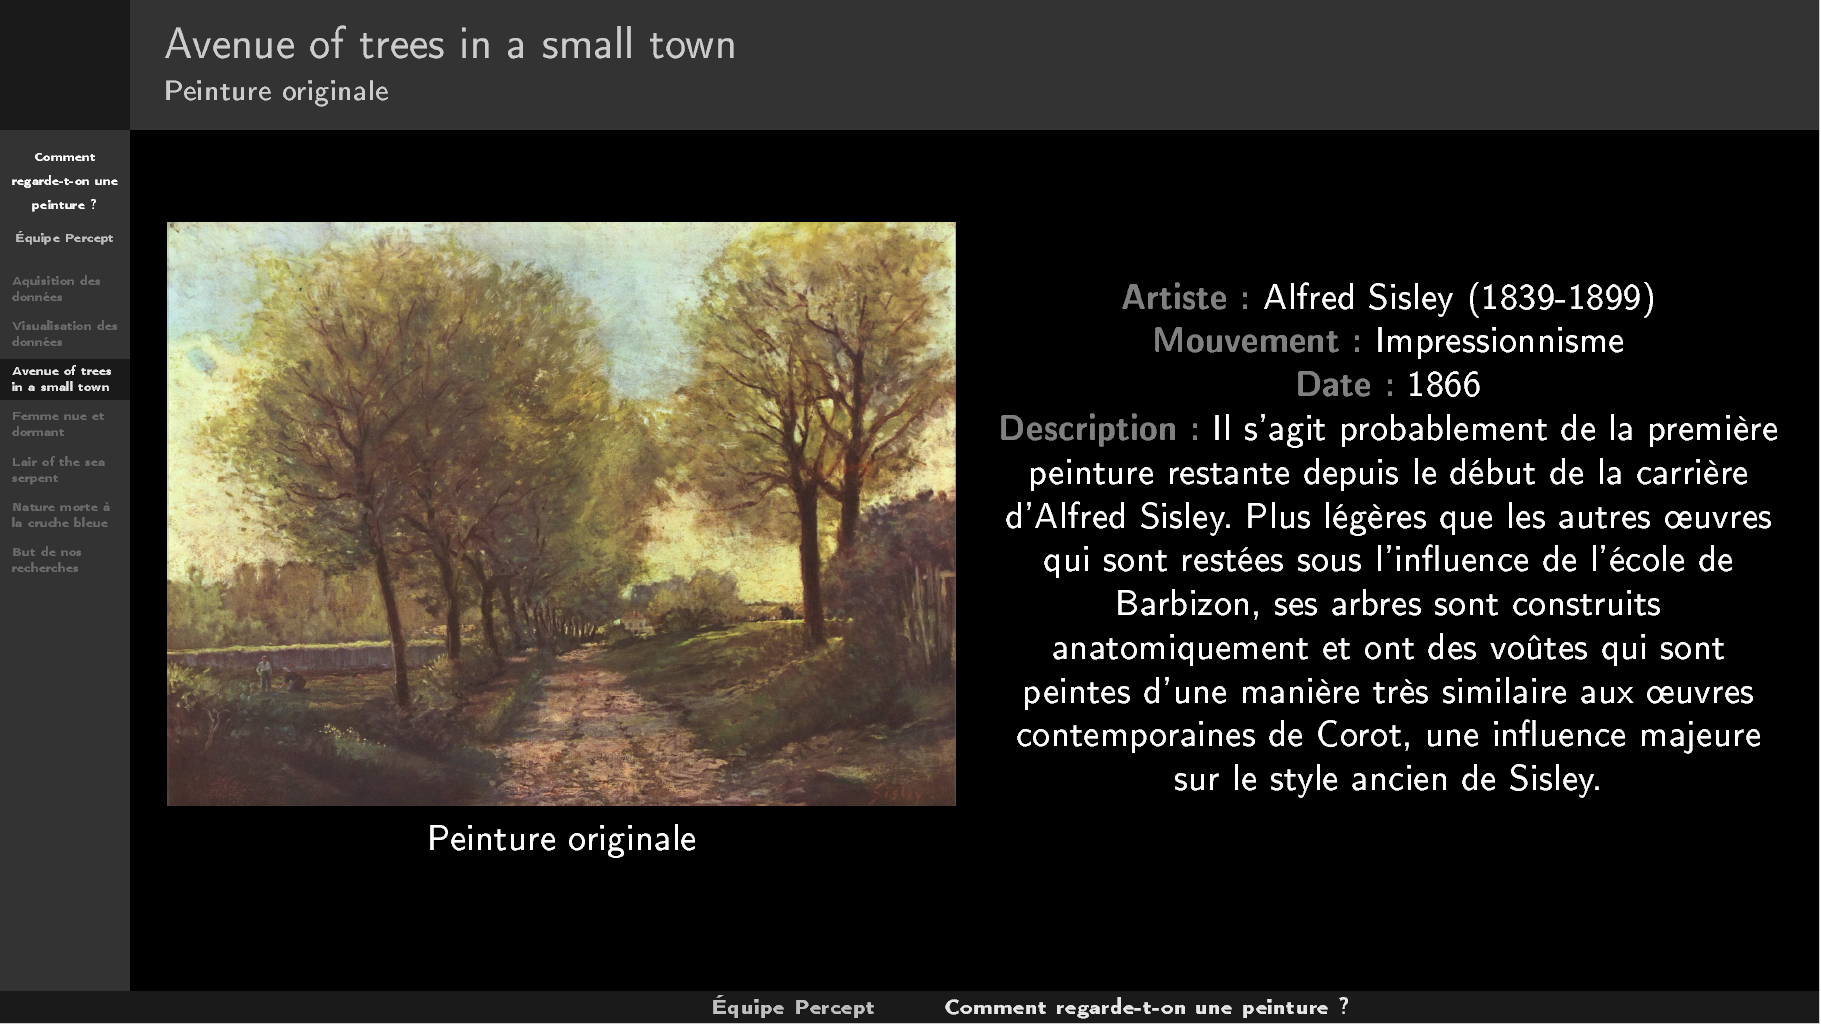
\includegraphics[width=0.7\linewidth]{datas/exemple_diapo.png}
    \caption{Extrait de la présentation}
    \label{ex_diapo}
\end{figure}

\par
Afin de rajouter des animations dans mon diaporama, notamment des vidéos pour faciliter la compréhension, je me suis lancé dans la programmation de petits programmes en langage Python. Même si il y a eu de nombreux TPs en Python lors de cette année à l'ESIR j'ai remarqué que j'avais encore beaucoup à apprendre en regardant ce qu'il se faisait déjà sur le gitlab de l'équipe Percept (site web qui permet d'échanger et de sauvegarder facilement des documents). Cela m'a aussi permis de me familiariser avec les différentes données présentes dans la base de données oculométriques.

\section{Vidéo fondue}

Le premier script permet de créer une vidéo avec une \textbf{transition en fondu} entre chaque image donnée en entrée du programme. L'intérêt d'un tel script est de le combiner au résultat d'un autre programme du gitlab qui donnait des cartes de chaleur de saillance. Ce sont des cartes de saillance en couleur où les zones saillantes sont représentées par des couleurs chaudes. Cela permet de faire évoluer la carte de chaleur de saillance en fonction du temps d'observation (voir Image \ref{fondu}). Pour ma présentation, j'ai généré des cartes de chaleur au bout de 1 seconde d'observation, puis au bout de 2, etc. jusqu'à 5 secondes d'observation. La vidéo permettait donc d'enchainer les différentes cartes de chaleur avec un rendu propre avec pour but final d'analyser l'évolution de la saillance au cours du temps.

\begin{figure}[!ht]
    \centering
    \begin{subfigure}{.3\textwidth}
        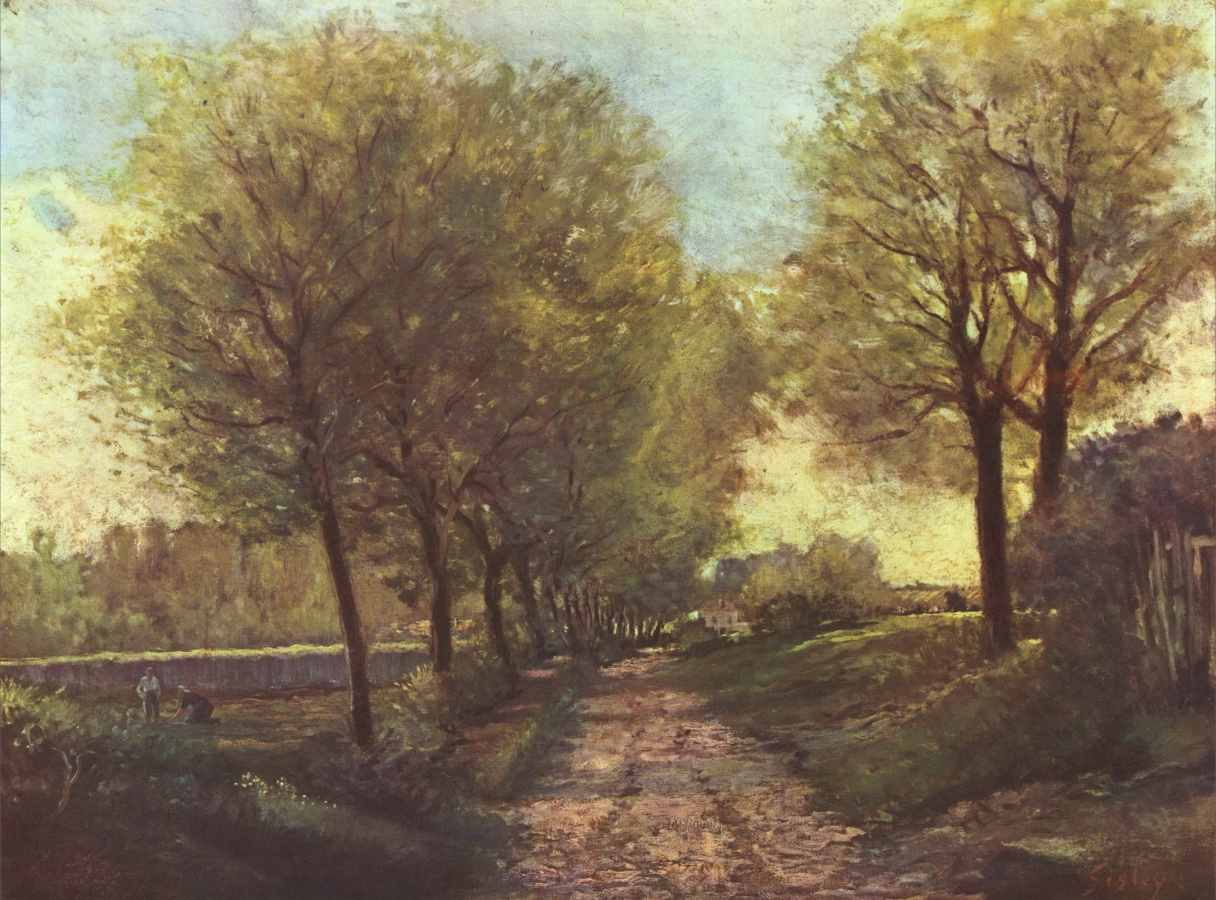
\includegraphics[width=\linewidth]{datas/fondu_00.jpg}
        \caption{}
    \end{subfigure}
    \begin{subfigure}{.3\textwidth}
        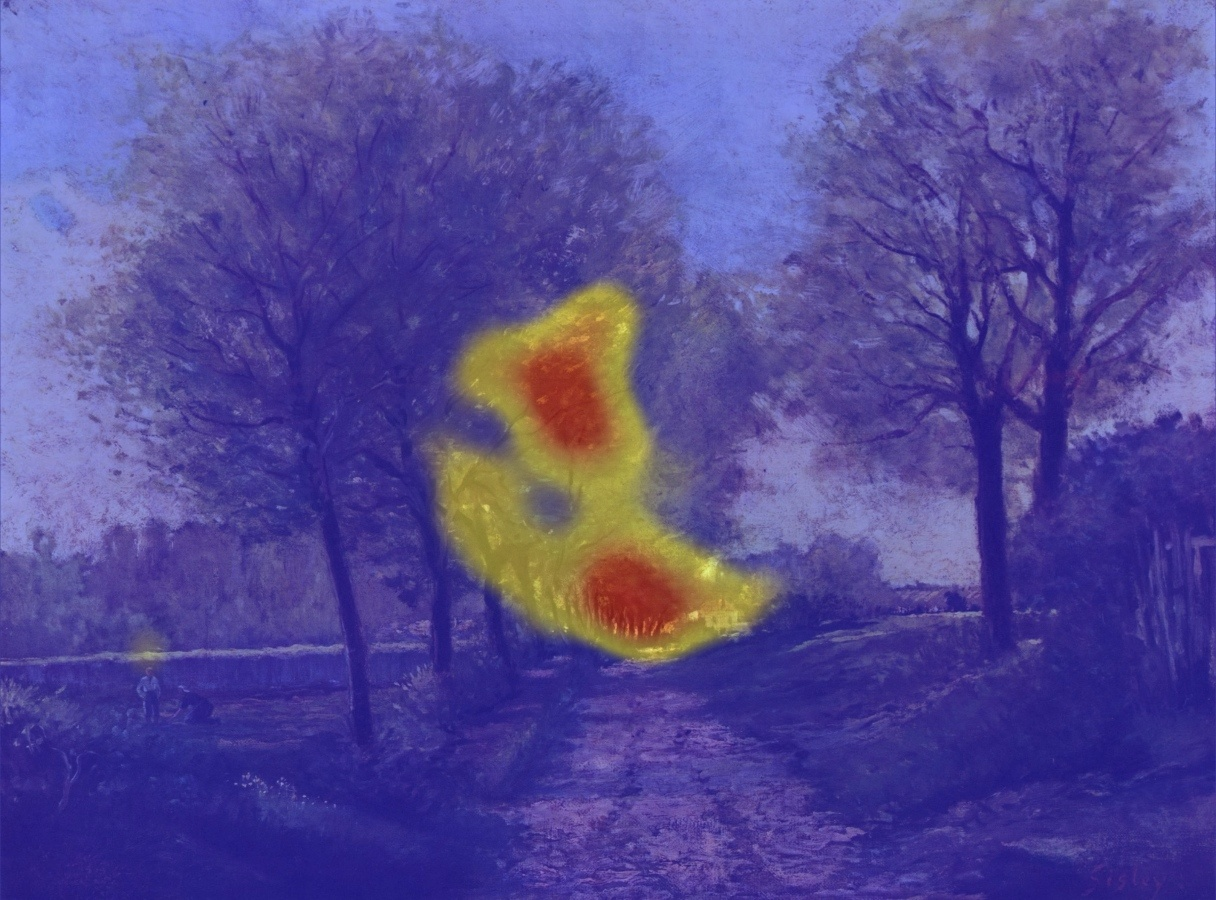
\includegraphics[width=\linewidth]{datas/fondu_02.jpg}
        \caption{}
    \end{subfigure}
    \begin{subfigure}{.3\textwidth}
        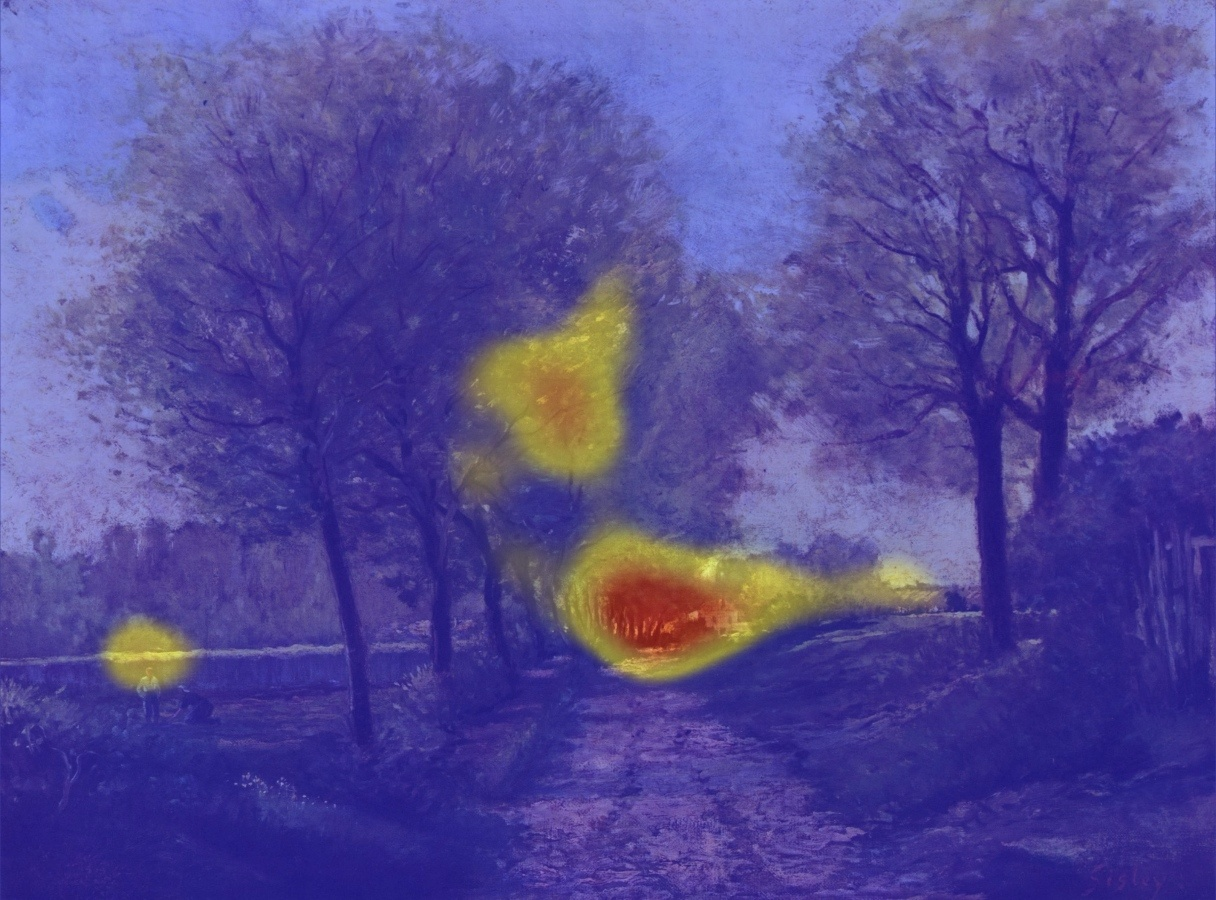
\includegraphics[width=\linewidth]{datas/fondu_05.jpg}
        \caption{}
    \end{subfigure}
    \caption{(a) Peinture originale, (b) Carte de chaleur de saillance après 2s d'observation, (c) Carte de chaleur de saillance après 5s d'observation}
    \label{fondu}
\end{figure}

\par
Ce programme n'est pas très compliqué en soit mais il m'a permis de découvrir des librairies sur Python très utiles que je n'avais jamais essayé auparavant.

\section{Vidéo chemins visuels}

Mon deuxième script consistait à afficher les chemins visuels réprésentés par des cercles et des lignes comme vu précédemment avec l'image \ref{ex_scanpath}. Cela permet de visualiser le mouvement des yeux de l'observateur et de pouvoir suivre son regard. Les défauts du résultat obtenu c'est que lorsqu'il y avait plusieurs observateurs l'image était rapidement surchargée par les chemins visuels qui se superposaient et les couleurs choisies aléatoirement pour différencier les observateurs pouvaient être très similaires.

\par
J'ai donc fait évoluer ce script en y ajoutant de l'animation. J'ai rajouté une option qui permettait de générer une vidéo où chaque cercle (donc chaque fixation) s'affichait les uns après les autres. Cela permet donc d'avoir en fin de vidéo une image qui reste surchargée mais comme le spectateur a suivi le déroulement de l'animation, celui-ci est beaucoup moins confus. Ce point est aussi vrai pour l'inconvénient des couleurs trop similaires.